\documentclass[11pt]{article}
\usepackage[margin=1in]{geometry}
\usepackage{amsmath,amssymb,amsthm}
\usepackage{booktabs}
\usepackage{tikz}
\usepackage[hidelinks]{hyperref}
\usepackage{url}

\newtheorem{proposition}{Proposition}
\newtheorem{remark}{Remark}
\newenvironment{plain}{\begin{quote}\small\noindent\textbf{In plain words.}~}{\end{quote}}

\title{Three Ways Across a Turn:\\ Chord, Arc and Tangent}
\author{Bee Rosa Davis\\ Davis Geometric}
\date{November 2026 \quad (working draft)}

\begin{document}
\maketitle

\begin{abstract}
When a unit segment turns through an angle $\theta$, its tip can be joined to where it
started in three natural ways: by the straight chord, by the arc the turn actually
traces, and by the two tangent lines that meet outside the circle. Their lengths are
$2\sin(\theta/2)$, $\theta$ and $2\tan(\theta/2)$, and they are always in that order. All
of this is classical, from Archimedes through Snellius and Huygens. This paper collects
what the three paths mean when the turn is read as a complex number $U=e^{i\theta}$ or a
unit quaternion. The chord is $U-1$, and its square is Wilson's lattice energy. The arc is
the logarithm, and its square is the continuum energy. The tangent leg $\tan(\theta/2)$ is
the Cayley parameter that builds $U$ algebraically, and read as a time step it is the
Crank--Nicolson rule. The chord and the tangent miss the arc in opposite directions, the
tangent by exactly twice as much at leading order. So the Snellius--Huygens weights
$2{:}1$ cancel the leading error both in length and in energy: $(2C^2+T^2)/3=\theta^2+
\tfrac{7}{720}\theta^6+\dots$. Half the chord is the distance $d$ of the identity $S+d^2=1$,
with sameness $S=\cos^2(\theta/2)$. On the $SU(2)$ meshes of our curvature-recovery work,
face angles are small enough (at most $0.094$) that the chord and the arc differ in energy
by under $0.08\%$, so these corrections are not the source of the errors measured there.
Every miss has a twin on the other side, and crossing the circle's rim makes the turn
imaginary while $S+d^2=1$ survives. Bertrand's paradox turns out to be the question of
which of these quantities is taken to be uniform: the arc, $\sqrt S$, or $S$.
Every identity is checked symbolically or numerically by a script that ships with the paper.
\end{abstract}

\section{A picture}\label{sec:picture}

Draw a line of length one from the origin to the point $1$. Turn it through an angle
$\theta$. Its tip moves along the unit circle from $1$ to $e^{i\theta}$. Turn it in every
direction and the tip traces the whole circle.

Now ask the two positions of the tip to reach each other again. There are three natural
ways (Figure~\ref{fig:three}). The \emph{chord} goes straight through the circle. The
\emph{arc} goes along the circle, the way the turn went. The \emph{outside path} follows the
tangent line at one end to the point where it meets the tangent at the other, and then
comes back in. The arc is the only one of the three that the turn itself can travel; the
chord is the shortcut that cuts across, and the outside path is the detour that never
touches the circle in between.

\begin{plain}
Turning a stick through an angle moves its tip along a curve. Afterwards the two tip
positions can be joined by cutting straight across (the chord), by going around the way
the stick went (the arc), or by going out along the two edge lines and back (the outside
path). The shortcut is always shortest and the detour always longest. The true path lies
between them. This paper is about what each of the three means, and what it costs.
\end{plain}

\begin{figure}[t]\centering
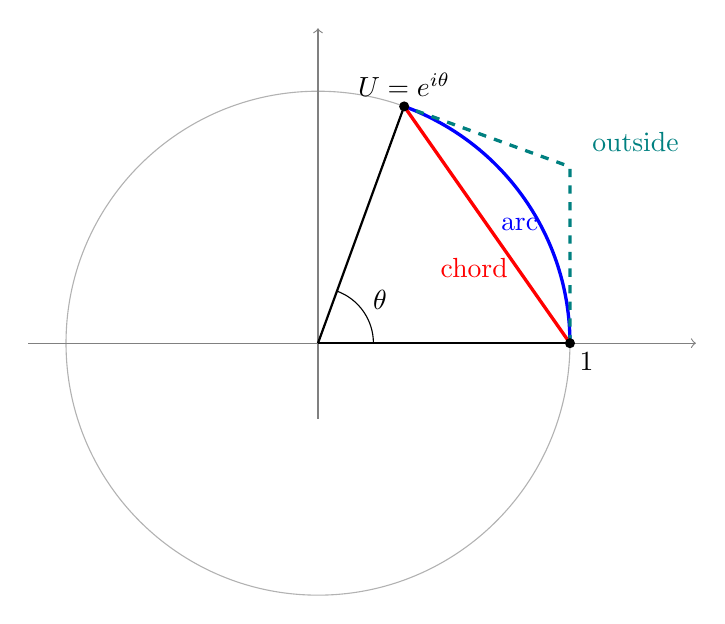
\begin{tikzpicture}[scale=3.2]
  \def\t{70}
  \draw[gray!60] (0,0) circle (1);
  \draw[->,gray] (-1.15,0) -- (1.5,0);
  \draw[->,gray] (0,-0.3) -- (0,1.25);
  \draw[thick] (0,0) -- (1,0);
  \draw[thick] (0,0) -- ({cos(\t)},{sin(\t)});
  \draw[very thick,blue] (1,0) arc (0:\t:1);
  \draw[very thick,red] (1,0) -- ({cos(\t)},{sin(\t)});
  \coordinate (Q) at ({1/cos(\t/2)*cos(\t/2)},{1/cos(\t/2)*sin(\t/2)});
  \draw[very thick,teal,dashed] (1,0) -- (Q) -- ({cos(\t)},{sin(\t)});
  \draw (0.22,0) arc (0:\t:0.22); \node at ({0.3*cos(\t/2)},{0.3*sin(\t/2)}) {$\theta$};
  \fill (1,0) circle (0.02) node[below right] {$1$};
  \fill ({cos(\t)},{sin(\t)}) circle (0.02) node[above] {$U=e^{i\theta}$};
  \node[red] at (0.62,0.30) {chord};
  \node[blue] at (0.80,0.47) {arc};
  \node[teal] at (1.26,0.80) {outside};
\end{tikzpicture}
\caption{Three ways across a turn of $\theta=70^\circ$: the chord (length $2\sin(\theta/2)$),
the arc ($\theta$) and the outside path along the two tangents ($2\tan(\theta/2)$).}
\label{fig:three}
\end{figure}

Write $C=2\sin(\theta/2)$, $A=\theta$ and $T=2\tan(\theta/2)$ for the three lengths. The
outside corner lies on the bisector at distance $\sec(\theta/2)$ from the centre, so each
tangent segment has length $\tan(\theta/2)$.

\paragraph{What is classical, and what this paper adds.} The inequality $C<A<T$ is
Archimedes' squeeze of the circle between inscribed and circumscribed polygons
\cite{archimedes}. The weighted combination of Section~\ref{sec:lengths} is the
Snellius--Huygens estimate \cite{snellius,huygens}. The chord energy is Wilson's lattice
action \cite{wilson}, the arc energy is Manton's \cite{manton}, the Cayley map is from
1846 \cite{cayley}, and Crank--Nicolson is from 1947 \cite{cn}. None of these
identifications is new. What this paper does is read the three paths as one object: three
ways of measuring the same turn, which miss in fixed proportions, with each proportion
showing up again in energy, in algebra and in time stepping. It then checks how much
this matters on a real non-Abelian mesh. The energy combination of
Section~\ref{sec:energy} is the one statement we have not found in the sources above. A
proper prior-art search is listed as open in Section~\ref{sec:claims}.

\section{Lengths: who misses, and by how much}\label{sec:lengths}

\begin{proposition}\label{prop:lengths}
For $0<\theta<\pi$, $C<A<T$, and
\[
A-C=\tfrac{1}{24}\theta^3+O(\theta^5),\qquad T-A=\tfrac{1}{12}\theta^3+O(\theta^5).
\]
The outside path overshoots by exactly twice what the chord falls short, at leading order. Hence
\[
\frac{2C+T}{3}=\theta+\tfrac{1}{320}\theta^5+O(\theta^7),
\]
and $(2C+T)/3>\theta$ on the whole interval (the Snellius--Huygens inequality
$2\sin x+\tan x>3x$ for $0<x<\pi/2$, with $x=\theta/2$).
\end{proposition}
\begin{proof}
The series follow from $\sin x=x-x^3/6+x^5/120-\dots$ and $\tan x=x+x^3/3+2x^5/15+\dots$ at
$x=\theta/2$. The inequalities are classical \cite{archimedes,huygens}; all are checked by
\texttt{verify.py}.
\end{proof}

\begin{plain}
The shortcut falls short of the true path, and the detour overshoots it. For small turns
the overshoot is always exactly twice the shortfall. So if you take the shortcut twice and
the detour once and average, the two errors cancel, and you get the true length almost
perfectly: the leftover error shrinks like the fifth power of the angle. Snellius found
this in 1621 and Huygens proved it in 1654. Neither side alone tells the truth; the two
sides together nearly do.
\end{plain}

\section{The turn as a number}\label{sec:number}

Read the turn as the complex number $U=e^{i\theta}$. Then the chord is the complex
number $U-1$, and
\[
U-1=2i\sin(\theta/2)\,e^{i\theta/2}.
\]
Its length is $C$, and its direction is the starting direction turned by $\theta/2$ (plus
a quarter turn). \emph{The chord turns at half the speed of the line.} Turning the line
once around, $\theta=2\pi$, turns the chord's direction only half way.

\paragraph{The chord and sameness.} Write
\[
S=\cos^2(\theta/2)=\tfrac12(1+\operatorname{Re}U),\qquad d=\sin(\theta/2)=\tfrac12 C.
\]
Then $S+d^2=1$, and $1-S=C^2/4$. This is the identity of the double-cover paper
\cite{davis-dc}, with $d$ read as half the chord and $S$ as the sameness of the two
positions. Two positions are fully the same ($S=1$) when the chord vanishes. They are
fully different ($S=0$) at the half turn, where the chord is a diameter.

\paragraph{The tangent and the Cayley map.} The tangent leg $\tau=\tan(\theta/2)$ builds
the turn algebraically, with no exponential:
\[
U=\frac{1+i\tau}{1-i\tau},\qquad
\tau=\frac{\sin\theta}{1+\cos\theta}=\frac{\operatorname{Im}U}{1+\operatorname{Re}U}=
\frac{\operatorname{Im}U}{2S}.
\]
This is the Cayley transform \cite{cayley}. As $\theta\to\pi$, $\tau\to\infty$: at the half
turn the two tangents are parallel, never meet, and the outside path has no corner. The
Cayley map reaches every turn except the half turn.

\begin{plain}
As a number, the turn is a point on the unit circle. The shortcut is ``where you are
minus where you started''. Its direction turns half as fast as the stick does, which is
why one full turn of the stick only half-turns the shortcut. Half the shortcut's length is
exactly the distance $d$ in the double-cover identity $S+d^2=1$, so the shortcut measures
how different the two positions are. The detour's leg is the one number that rebuilds the
whole turn with only arithmetic, no exponentials. At a half turn it breaks: the two edge
lines are parallel and never meet.
\end{plain}

\section{Energy}\label{sec:energy}

In lattice gauge theory the turn $U$ is the holonomy around a face, and the face's
energy measures how far $U$ is from $1$ \cite{wilson}. Each of the three paths gives an
energy:
\[
C^2=2(1-\cos\theta)=\theta^2-\tfrac{1}{12}\theta^4+\tfrac{1}{360}\theta^6-\dots,\qquad
A^2=\theta^2,\qquad
T^2=\theta^2+\tfrac16\theta^4+\tfrac{17}{720}\theta^6+\dots
\]
$C^2$ is Wilson's action (up to normalisation), and $A^2$ is Manton's geodesic action
\cite{manton}, which is the continuum energy of the face. The tangent energy again misses on
the other side, and again by exactly twice as much at leading order. So the same
Snellius--Huygens weights cancel it.

\begin{proposition}\label{prop:energy}
\[
\frac{2C^2+T^2}{3}=\theta^2+\tfrac{7}{720}\theta^6+\tfrac{1}{1008}\theta^8+O(\theta^{10}).
\]
The $\theta^4$ term cancels exactly. The combination is algebraic in $U$:
$C^2=|U-1|^2$ and $T^2=4\,|\operatorname{Im}U|^2/(1+\operatorname{Re}U)^2$.
\end{proposition}

\begin{plain}
The energy of a turn can be measured with the shortcut, the true path or the detour.
Lattice physics has used the shortcut since 1974 because it is easy to compute; the true
path is what the continuum means. The shortcut energy is slightly too small and the detour
energy slightly too big, by twice as much. Mixing them two-to-one cancels the main error,
using only arithmetic on $U$.
\end{plain}

\begin{remark}[What this does and does not correct]
On a lattice of spacing $a$ and a smooth field, $\theta=O(a^2)$, so the $\theta^4$ term is a
relative correction of order $a^4$. The dominant lattice error is of order $a^2$ and comes
from the shape of the face, not from the compactness of the group; it is what Symanzik
improvement removes \cite{lw}. The combination above addresses only the compactness error.
That error matters for strong fields and coarse lattices, and is negligible for smooth
fields on fine ones. The tangent energy also diverges at the half turn $U=-1$, unlike
Wilson's and like the Cayley map. Whether that barrier is harmless or harmful in a lattice
simulation is not studied here.
\end{remark}

\section{The non-Abelian turn}\label{sec:su2}

A unit quaternion (an element of $SU(2)$) is $U=\cos a+n\sin a$ with $n$ a pure unit
quaternion. Everything above carries over with $\theta$ replaced by the geodesic angle $a$
on $S^3$:
\[
|U-1|=2\sin(a/2),\qquad \log U=a\,n,\qquad
U=(1+v)(1-v)^{-1}\ \text{with}\ v=\frac{\operatorname{Im}U}{1+\operatorname{Re}U},\ |v|=\tan(a/2).
\]
The quaternion $U$ rotates three-space by $2a$, so the chord, arc and outside path of the
quaternion live on the double cover of the rotation they describe. The Cayley vector $v$
again reaches everything except $U=-1$, the other sheet's copy of the identity.
\texttt{verify.py} checks all three on $2{,}000$ random quaternions. The chord and arc
agree to $10^{-14}$. The Cayley reconstruction agrees to $10^{-10}$; its conditioning
grows like $1/(1+\cos a)$ near the half turn.

\begin{plain}
The same three paths exist for turns in three dimensions, written as quaternions. The
formulas are identical with the turning angle measured on the three-sphere. The detour
still rebuilds the turn with plain arithmetic, and it still breaks only at the half turn.
\end{plain}

\section{Time stepping}\label{sec:time}

Take the simplest motion that turns: $y'=i\,y$, whose exact solution goes around the
circle. One step of size $s$ should turn $y$ by $s$. The three classical one-step rules put
the point in three places, and they are the three paths again.

\begin{itemize}
  \item \textbf{Explicit Euler}, $y\mapsto(1+is)\,y$, steps out along the tangent line. Its
    modulus is $\sqrt{1+s^2}>1$, so it leaves the circle outward and gains energy every step.
  \item \textbf{Implicit Euler}, $y\mapsto y/(1-is)$, has modulus $1/\sqrt{1+s^2}<1$. It falls
    inside the circle and loses energy every step.
  \item \textbf{Crank--Nicolson}, $y\mapsto\frac{1+is/2}{1-is/2}\,y$, is the Cayley map with
    $\tau=s/2$. It stays exactly on the circle, but turns by $\varphi=2\arctan(s/2)$. The step
    $s$ plays the role of the outside path $T$, and the turn actually made is the arc. The
    phase lag is $s-\varphi=\tfrac{1}{12}s^3+O(s^5)$, the same $1/12$ as $T-A$ in
    Proposition~\ref{prop:lengths}.
\end{itemize}

For a general linear flow $y'=-Gy$, the Crank--Nicolson factor
$r(z)=(1-z/2)/(1+z/2)$ satisfies $|r(z)|\le1$ exactly when $\operatorname{Re}z\ge0$. Its
behaviour on a non-normal $G$ is controlled by the numerical range $W(G)$. By
Crouzeix--Palencia \cite{cp}, $\|r(hG)^k\|\le(1+\sqrt2)\sup_{z\in W(G)}|r(hz)|^k$. On a Lie
group, the Cayley map keeps each update exactly on $SU(2)$ \cite{iserles}.

\begin{plain}
Simulating something that spins means stepping it forward a little at a time. The plainest
step walks out along the edge line and drifts outward, gaining energy it should not have.
The backward version drifts inward and loses energy. The Cayley step, the detour's leg, stays
exactly on the circle and only lags a little behind, by the same one-twelfth that separates
the detour from the true path. For our next step, simulating the flow on the mesh, that is
the natural rule to try first. The numerical range we are measuring tells us how big its
steps may be.
\end{plain}

\section{Twins, the far side, and Bertrand}\label{sec:twins}

\paragraph{Every miss has a twin on the other side.} The Snellius--Huygens estimate
$(2C+T)/3$ overshoots the arc. Snellius' other estimate undershoots it:
\[
L=\frac{6\sin(\theta/2)}{2+\cos(\theta/2)},\qquad
\theta-L=\tfrac{1}{2880}\theta^5+O(\theta^7),\qquad L<\theta<\frac{2C+T}{3}.
\]
The two misses are $\theta^5/320$ above and $\theta^5/2880$ below, nine to one. So the twins
can be blended again, $\tfrac{1}{10}\bigl(9L+\tfrac{2C+T}{3}\bigr)=\theta+O(\theta^7)$, and the
blend leaves a smaller pair of twins. Each cancellation produces the next.

\paragraph{The far-side twin.} A chord does not know which way round the turn went. The
turns $\theta$ and $2\pi-\theta$ have the same chord. The outside path does know: its
tangent leg changes sign, $\tan\bigl((2\pi-\theta)/2\bigr)=-\tan(\theta/2)$, because the
corner where the tangents meet moves to the other side of the circle.

\paragraph{Where the corner sits.} The chord's line lies at distance $p=\cos(\theta/2)$
from the centre, and the corner at distance $1/p$ (pole and polar). The corner's
position decides the regime.
\begin{itemize}
  \item \emph{Corner outside the circle} ($0<p<1$): everything is real.
  \item \emph{Chord line through the centre} ($p=0$, the half turn): the tangents are
    parallel and the corner is at infinity. Past it, the corner comes back on the far side;
    that is the far-side twin. Crossing the centre flips to the twin, and everything stays real.
  \item \emph{Corner inside the circle} ($p>1$; the chord's line misses the circle): the
    two endpoints become a complex-conjugate pair, and the turn becomes imaginary,
    $\theta=i\varphi$. Then $C=2i\sinh(\varphi/2)$, the tangent leg is $i\tanh(\varphi/2)$, and
    $S=\cosh^2(\varphi/2)>1$. The identity $S+d^2=1$ survives, with $d=i\sinh(\varphi/2)$
    imaginary. The circle has become a hyperbola, and the turn a boost. Crossing the rim is
    what makes the numbers unreal.
\end{itemize}

\paragraph{Bertrand's paradox.} Bertrand asked for the probability that a ``random chord''
is longer than the side of the inscribed equilateral triangle \cite{bertrand}. The answer
depends on how the chord is chosen, and each classical choice makes one of this paper's
quantities uniform:
\begin{center}\small
\begin{tabular}{lll}\toprule
Chord chosen by & Uniform quantity & Probability \\ \midrule
two random endpoints & the arc $\theta$ & $1/3$ \\
random distance along a radius & $\sqrt S=\cos(\theta/2)$ & $1/2$ \\
random midpoint & the sameness $S$ & $1/4$ \\
\bottomrule\end{tabular}
\end{center}
The chord exceeds $\sqrt3$ exactly when $\theta>2\pi/3$, $\cos(\theta/2)<1/2$ and $S<1/4$, so
the three answers follow at once. A simulation with two million chords per method gives
$0.3333$, $0.5004$ and $0.2498$. The outside path offers no fourth answer: its leg runs off to
infinity at the half turn, so it cannot be spread evenly. Jaynes argued that invariance
under moving and rescaling the circle selects the radius method \cite{jaynes}.

\begin{plain}
Every estimate that misses on one side has a twin that misses on the other, and blending
the twins cancels the miss, leaving a smaller pair. A chord also has a twin turn: the long
way around gives the same chord, but the detour notices, because its corner jumps to the
other side. Where that corner sits decides everything. Outside the circle, all is real.
Through the centre, you flip to the twin. Inside the circle, the numbers become imaginary,
the circle becomes a hyperbola, and still $S+d^2=1$ holds. Bertrand's famous paradox is the
same question in disguise: ``random chord'' means nothing until you say which of these
quantities you are spreading evenly, the arc, the square root of sameness, or sameness
itself.
\end{plain}

\section{How much this matters on a real mesh}\label{sec:mesh}

Our curvature-recovery work measures an $SU(2)$ force on meshes of the Poincar\'e homology
sphere, at the Levi-Civita connection of a Berger metric. Its native action is the chord
energy: each face's defect is $D=U_f-1$. Table~\ref{tab:angles} gives the face angles $a$
on those meshes (\texttt{face\_angles.py}, from the frozen inputs).

\begin{table}[h!]\centering\small
\caption{Face holonomy angles on the $SU(2)$ Berger meshes, and the relative gap between
chord and arc energy at the largest angle, $a^2/12$.}
\label{tab:angles}
\begin{tabular}{rrrrr}\toprule
$n$ & faces & median $a$ & max $a$ & chord--arc energy gap at max \\ \midrule
1 & 480 & 0.0684 & 0.0937 & $7.3\times10^{-4}$ \\
2 & 3{,}840 & 0.0172 & 0.0250 & $5.2\times10^{-5}$ \\
3 & 12{,}960 & 0.0076 & 0.0113 & $1.1\times10^{-5}$ \\
5 & 60{,}000 & 0.0027 & 0.0041 & $1.4\times10^{-6}$ \\
\bottomrule\end{tabular}
\end{table}

The angles shrink roughly like the face area, and the chord--arc energy gap is below
$0.08\%$ everywhere. The force errors measured there are $2.5\%$ to $36\%$. So the
chord-versus-arc choice is not what limits that work, and the two readings used there
(the arc, through $\log U$, for the covariant recovery; the chord, $U-1$, for the force)
agree to well within the measured error. The three paths matter for that programme at
the next step instead: the time integrator of Section~\ref{sec:time}.

\begin{plain}
On the meshes we actually use, every face turns by less than a tenth of a radian. There the
shortcut and the true path differ in energy by less than a tenth of a percent, far smaller
than the errors we measure. So this idea does not explain those errors, and we say so. Where
it does matter is in simulating the motion over time, which is the next step of that work.
\end{plain}

\section{What is claimed, and what is open}\label{sec:claims}

\textbf{Claimed}, each checked by \texttt{verify.py} (all checks passing; count in \texttt{verify\_output.txt}):
\begin{itemize}
  \item the length ordering, the $1/24$ and $1/12$ misses, and the Snellius--Huygens residual $\theta^5/320$;
  \item the chord's half-angle direction, and $S+d^2=1$ with $d$ as half the chord;
  \item the Cayley construction in $\mathbb{C}$ and in the quaternions;
  \item the energy series and the cancellation of $\theta^4$ in $(2C^2+T^2)/3$;
  \item the three one-step rules' placement relative to the circle, and the Crank--Nicolson phase lag $s^3/12$;
  \item the lower twin's miss $\theta^5/2880$ and the $9{:}1$ blend, the far-side sign flip, the
    continuation through the rim with $S+d^2=1$ intact, and Bertrand's three answers.
\end{itemize}
The face angles of Table~\ref{tab:angles} are measured from frozen data.

\textbf{Not claimed.} No priority is claimed for any classical identity above. We do not claim that
the combined energy is a better lattice action; that would need simulations and the
treatment of the half-turn barrier. We do not claim that this explains any error in the
curvature-recovery work; Section~\ref{sec:mesh} shows it does not.

\textbf{Open.}
\begin{itemize}
  \item A prior-art search for the energy combination of Proposition~\ref{prop:energy} and
    for tangent-based lattice actions in general.
  \item A Cayley (Crank--Nicolson) time integrator for the $SU(2)$ flow, tested against
    exact trajectories, with its step size set by the numerical range.
  \item A strong-field or coarse-lattice test where $\theta$ is not small, the only regime
    where the energy combination could matter.
\end{itemize}

\paragraph{A future direction.} The unit sphere in one dimension is the pair $\{-1,+1\}$,
and in four it is $SU(2)$, whose centre is again $\{-1,+1\}$. A companion note follows
that thread toward the curvature of the gauge group and the Yang--Mills mass gap. It keeps
exact statements apart from the open link, which this paper does not claim. The note is
\path{docs/research/unit-curvature-2026-11-18.md} in the \textsc{gigi} repository.

\paragraph{Reproducibility.} \texttt{verify.py} and \texttt{face\_angles.py} in this
directory; the output of the first is saved as \texttt{verify\_output.txt}, of the second as
\texttt{face\_angles.json}.

\begin{thebibliography}{99}\small
\bibitem{archimedes} Archimedes, \emph{Measurement of a Circle}, in T.~L.~Heath (ed.), \emph{The Works of Archimedes}, Cambridge University Press, 1897.
\bibitem{snellius} W.~Snellius, \emph{Cyclometricus}, Leiden, 1621.
\bibitem{huygens} C.~Huygens, \emph{De circuli magnitudine inventa}, Leiden, 1654.
\bibitem{cayley} A.~Cayley, Sur quelques propri\'et\'es des d\'eterminants gauches, \emph{J.\ reine angew.\ Math.} 32 (1846) 119--123.
\bibitem{cn} J.~Crank, P.~Nicolson, A practical method for numerical evaluation of solutions of partial differential equations of the heat-conduction type, \emph{Proc.\ Cambridge Philos.\ Soc.} 43 (1947) 50--67.
\bibitem{wilson} K.~G.~Wilson, Confinement of quarks, \emph{Phys.\ Rev.\ D} 10 (1974) 2445--2459.
\bibitem{manton} N.~S.~Manton, An alternative action for lattice gauge theories, \emph{Phys.\ Lett.\ B} 96 (1980) 328--330.
\bibitem{lw} M.~L\"uscher, P.~Weisz, On-shell improved lattice gauge theories, \emph{Commun.\ Math.\ Phys.} 97 (1985) 59--77.
\bibitem{iserles} A.~Iserles, H.~Z.~Munthe-Kaas, S.~P.~N{\o}rsett, A.~Zanna, Lie-group methods, \emph{Acta Numerica} 9 (2000) 215--365.
\bibitem{cp} M.~Crouzeix, C.~Palencia, The numerical range is a $(1+\sqrt2)$-spectral set, \emph{SIAM J.\ Matrix Anal.\ Appl.} 38 (2017) 649--655.
\bibitem{bertrand} J.~Bertrand, \emph{Calcul des probabilit\'es}, Gauthier-Villars, Paris, 1889.
\bibitem{jaynes} E.~T.~Jaynes, The well-posed problem, \emph{Found.\ Phys.} 3 (1973) 477--492.
\bibitem{davis-dc} B.~R.~Davis, The Double Cover Principle, Zenodo, 2026, \url{https://doi.org/10.5281/zenodo.18895462}.
\end{thebibliography}
\end{document}
